\documentclass[11pt,twoside,a4paper]{article}
\usepackage[left=2cm,top=1cm,right=2cm,nohead,nofoot]{geometry}
\usepackage[utf8]{inputenc}
\usepackage{hyperref}
\usepackage{amssymb}
\usepackage{graphicx}
\begin{document}
\author{Jesse Niemistö \and Leo Muona}
\title{Game Engine Architecture: End-term project - Spring 2013 \\
       Technical documentation}

\maketitle

\section{Basic architecture}

The software can be split into two distinct subsystems that have been implemented; animation and physics. Animation subsystem handles skeletal animaition (aka forward kinematics), while the physics subsystem is an interface for interacting with 3rd-party physics engine.

Chapters below will take a more in-depth look at the subsystems.

\section{Animation subsystem}

First a lil intro to computer animation. Usually artists animate the characters by only animating the movement of the characters skeletons. This makes animating much easier, as characters might consist tens of thousands of vertices, but only a handful of bones, or joints. Artist only animates the keyframes of the charactes and the computer the fills the 'void', the empty spaces between keyframes, with method called interpolation. After artists have made these animations, they are saved to a file, which then can be read by a software. There might be an huge number of animations, and they all are typically used in different situations. For example when character stands it has different animation than when it is walking. Interpolation between different animations is called crossfade. 

In skeletor a Skeleton class presents a skeleton. Skeleton consists of joints. And these joints form a tree like structure that forms the skeleton. Joint knows it's parent and child joints, so joint knows if it is a leaf or root node. Also this tree like structure makes it easy to recursively traverse skeletons joints. 

SkeletonPose class reflects a single pose of the skeleton in some given time. SkeletonPose class includes a set of transformations for each joint of the skeleton, which are applied to skeletons bind pose to make the pose. This means that only SkeletonPose class is changes when making poses. SkeletonPose class also includes function for crossfading between different animations (poses). The only assumption here is that skeletons that are crossfaded are identical.

COLLADA is an open standard XML schema for exchaning digital assets between various graphics software applications. Skeletor is able to read COLLADA-files with skeletons and animations. Actually only those datas are read as rest are ignored. 

\begin{figure}
  \centering
    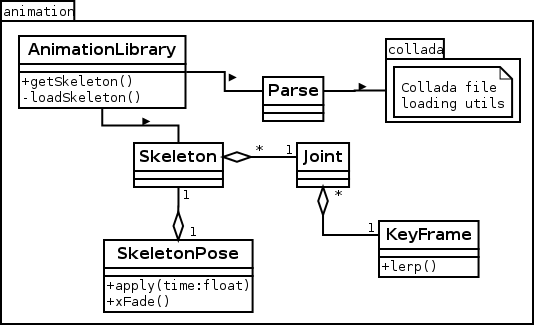
\includegraphics[scale=0.7]{animation_subsystem.png}
  \caption{animation subsystem architecture}
  \label{animsubsys}
\end{figure}

The figure in ~\ref{animsubsys} shows the basic architecture of the animation subsystem. The figure represents the classes defined under src/animation/ directory. Collada file structure is outside the scope of this document, but excellent tutorial is available for example in \url{http://www.wazim.com/Collada_Tutorial_1.htm}

\section{Physics subsystem}

Put your stuff in here Leorio~


\section{Known bugs and limitations}

Here is the list of known bugs and limitations on the software.

\begin{itemize}
  \item Collada
  \begin{itemize}
    \item Collada files must have at least and at most one skeleton.
    \item Root joint of the skeleton must be named as 'root'.
    \item Only Maya and blender exported collada files work and has been tested.
    \item Only library\_animation and library\_visual\_scene nodes are read, meaning character meshes are not read nor rendered.
    \item Only supported (and tested) version of collada schema is 1.4.1. Other versions are untested.
  \end{itemize}
  \item Animation crossfading only works with identical skeletons.
  \item KeyFrame animation assumes that interpolation is linear, no bezier is supported.
  \item Turning camera too far up or down distorts the scene, proper way of handling would be to put degrees of freedom to camera movement.
\end{itemize}

\end{document}
